% Digital Logic Lab 2
% Created: 2020-01-29 Sebastian Lopez - Megan Gordon 

%==========================================================
%=========== Document Setup  ==============================

% Formatting defined by class file
\documentclass[11pt]{article}

% ---- Document formatting ----
\usepackage[margin=1in]{geometry}	% Narrower margins
\usepackage{booktabs}				% Nice formatting of tables
\usepackage{graphicx}				% Ability to include graphics

%\setlength\parindent{0pt}	% Do not indent first line of paragraphs 
\usepackage[parfill]{parskip}		% Line space b/w paragraphs
%	parfill option prevents last line of pgrph from being fully justified

% Parskip package adds too much space around titles, fix with this
\RequirePackage{titlesec}
\titlespacing\section{0pt}{8pt plus 4pt minus 2pt}{3pt plus 2pt minus 2pt}
\titlespacing\subsection{0pt}{4pt plus 4pt minus 2pt}{-2pt plus 2pt minus 2pt}
\titlespacing\subsubsection{0pt}{2pt plus 4pt minus 2pt}{-6pt plus 2pt minus 2pt}

% ---- Hyperlinks ----
\usepackage[colorlinks=true,urlcolor=blue]{hyperref}	% For URL's. Automatically links internal references.

% ---- Code listings ----
\usepackage{listings} 					% Nice code layout and inclusion
\usepackage[usenames,dvipsnames]{xcolor}	% Colors (needs to be defined before using colors)

% Define custom colors for listings
\definecolor{listinggray}{gray}{0.98}		% Listings background color
\definecolor{rulegray}{gray}{0.7}			% Listings rule/frame color

% Style for Verilog
\lstdefinestyle{Verilog}{
	language=Verilog,					% Verilog
	backgroundcolor=\color{listinggray},	% light gray background
	rulecolor=\color{blue}, 			% blue frame lines
	frame=tb,							% lines above & below
	linewidth=\columnwidth, 			% set line width
	basicstyle=\small\ttfamily,	% basic font style that is used for the code	
	breaklines=true, 					% allow breaking across columns/pages
	tabsize=3,							% set tab size
	commentstyle=\color{gray},	% comments in italic 
	stringstyle=\upshape,				% strings are printed in normal font
	showspaces=false,					% don't underscore spaces
}

% How to use: \Verilog[listing_options]{file}
\newcommand{\Verilog}[2][]{%
	\lstinputlisting[style=Verilog,#1]{#2}
}




%======================================================
%=========== Body  ====================================
\begin{document}

\title{ELC 2137 Lab \# 2: Transistor Logic Gates}
\author{Sebastian Lopez - Megan Gordon}

\maketitle


\section*{Summary}

In this lab we described how logic gates are based on switches and how transistors behave like controllable switches. We also developed a circuit on a breadboard using standard electrical components, meanwhile also verifying the operation of a circuit.  

\section*{Deliverables}


	\begin{table}[ht]\centering
		\caption{Final Gate Logic/truth Table}
		\label{tbl:Logic_Truth_Table}
		\begin{tabular}{cc|c}
			\toprule
			Switch A & Switch B & A AND B \\
			\midrule
			0 & 0 & 0 \\
			0 & 1 & 0 \\
			1 & 0 & 0 \\
			1 & 1 & 1 \\
			\bottomrule
		\end{tabular} 
	\end{table} 
\section*{}

The logic operation that is implemented by the final gate is the AND operation due to the fact that both switches must be on in order for the LED to turn on as well. For an AND operator, an operator only returns a value of true if both of its opperands are true.  
	
	\begin{figure}[ht]\centering
		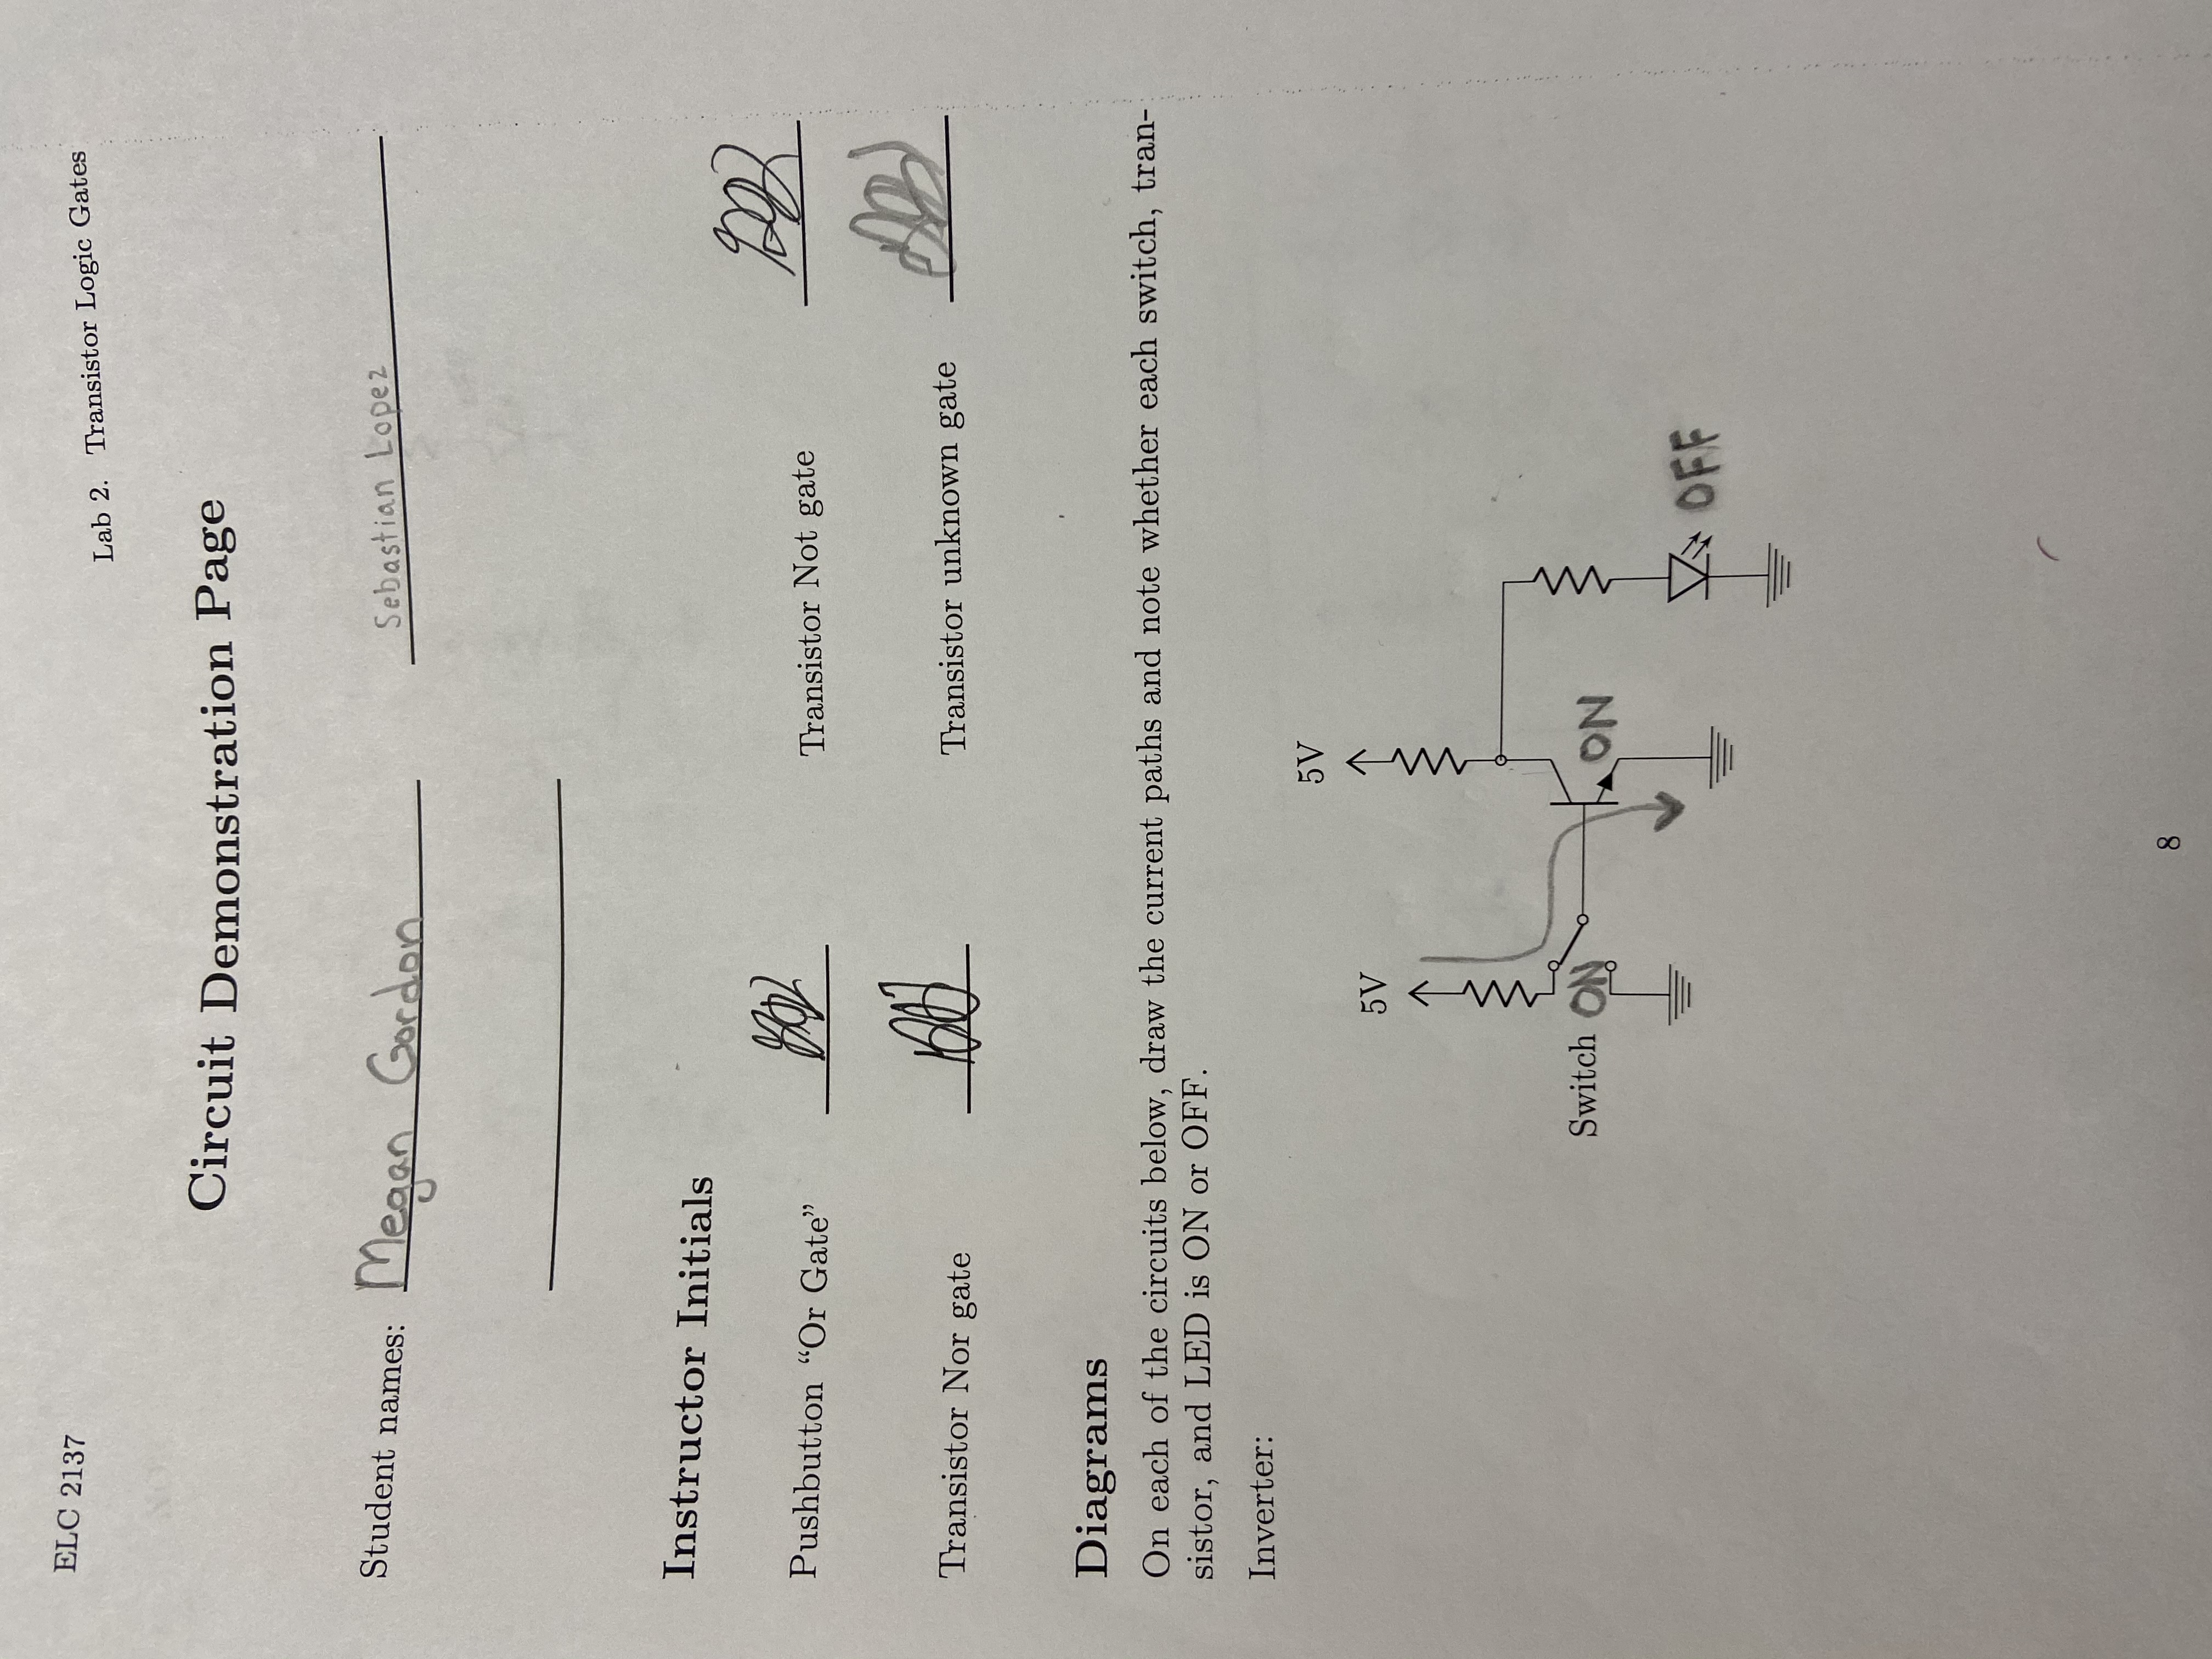
\includegraphics[width=\textwidth, angle=270 ,trim=50 50 50 50,clip]{Inverter_Gate}
		\caption{This is the picture of the Inverter Gate Diagram.}
		\label{fig:Inverter_Gate}
	\end{figure}
	
	\begin{figure}[ht]\centering
		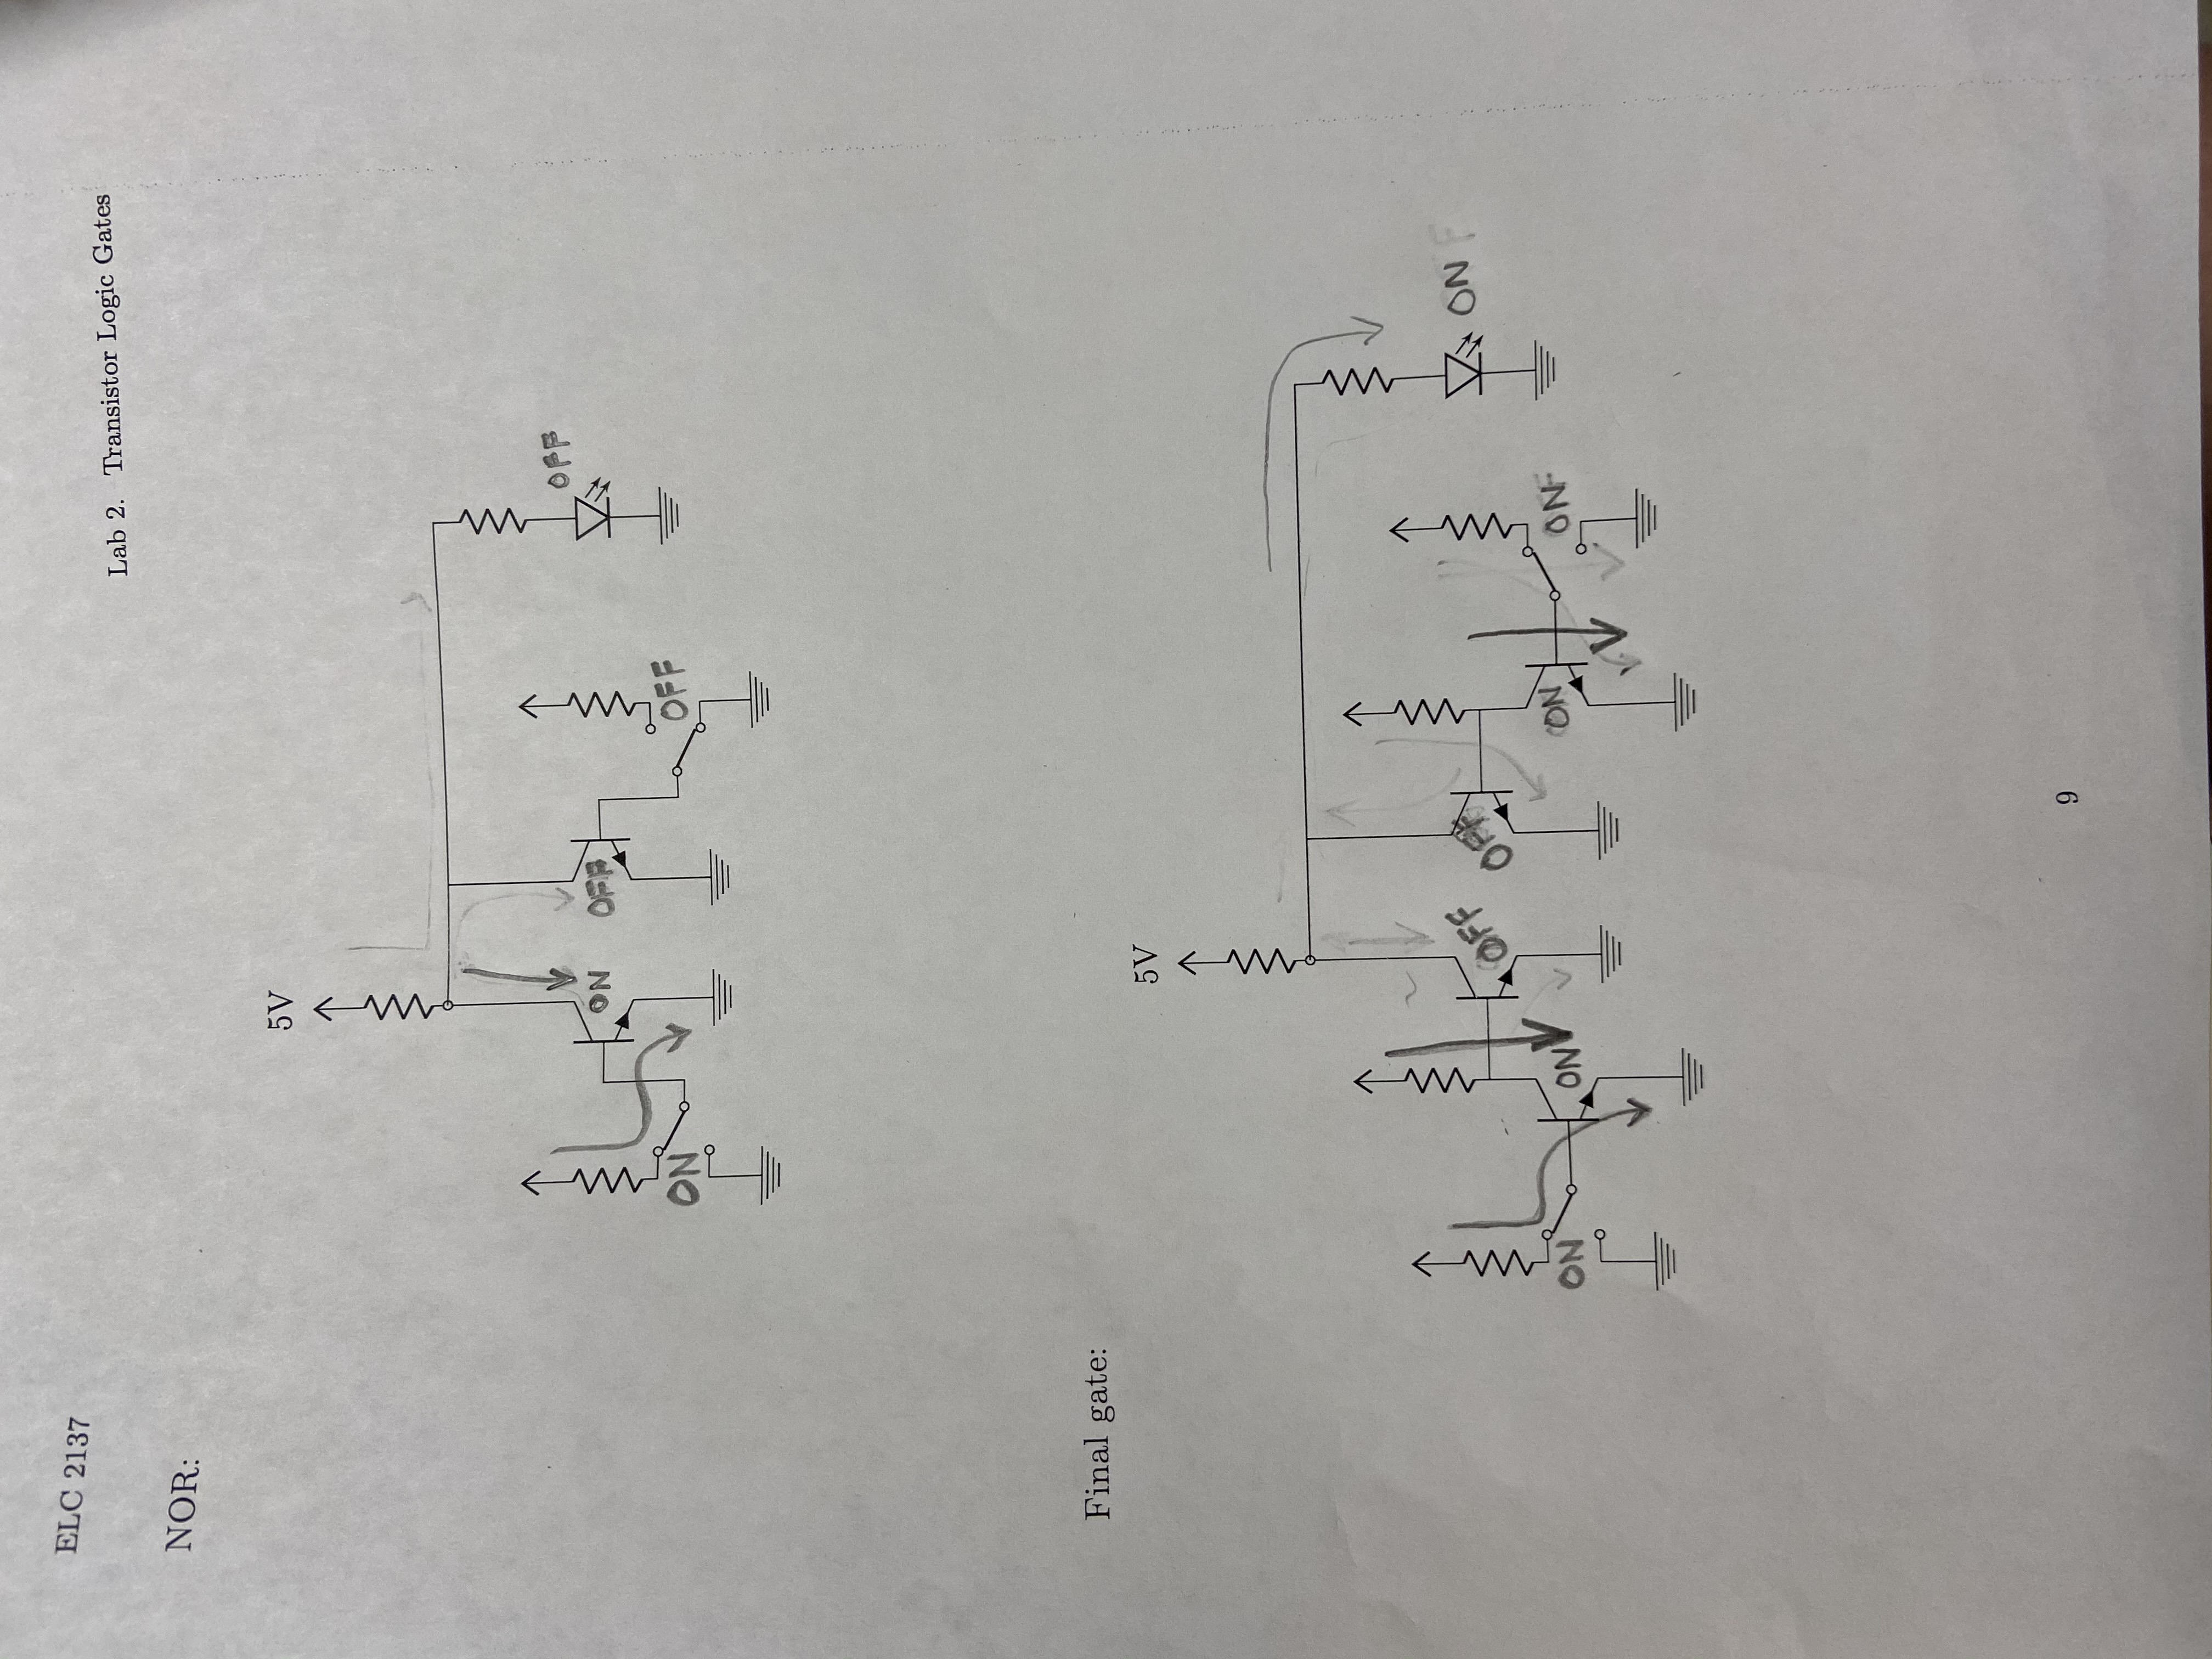
\includegraphics[width=\textwidth, angle=270 ,trim=50 50 50  50,clip]{NOR_Final_Gate}
		\caption{This is the picture of the NOR and the Final Gate Diagram.}
		\label{fig:NOR_Final_Gate}
	\end{figure}


\end{document}
